

For each cluster we sum the $K$-corrected $B$-band luminosity of all
galaxies brighter than the detection limit $z_{850} = 24.72$.  To
reduce noise, we discard galaxies that are clearly too bright to be
cluster members. In clusters with a central dominant (cD) galaxy or
dominant (but not central) brightest cluster galaxy(BCG), the bright
cutoff magnitude is set to the magnitude of the cD galaxy or BCG. In
clusters lacking a clearly dominant galaxy, we conservatively set the
cutoff based on the absolute magnitude of the most luminous cD galaxy
in any cluster, $M_B = -23.42$ (from cluster XMMU J2235.3$-$2557). The
bright cutoff magnitude in the observer frame, $z_{850}^{\rm bright}$,
is listed for each cluster in Table~\ref{tab:lum_params}.  Because
the bright cutoff is chosen so conservatively, we expect that no
cluster galaxies are discarded. The effect of being overly
conservative is only to add noise, and this is captured in the
statistical uncertainty described below.

For each cluster we apply the same selection criteria and
$K$-corrections to the GOODS fields to determine the ``background''
specific to that cluster. The GOODS fields
consist of a North field centered at approximately $\alpha = 12^{\rm
h} 36^{\rm m}$, $\delta = +62^{\circ} 14'$ and a South field centered
at approximately $\alpha = 3^{\rm h} 32^{\rm m}$, $\delta =
-27^{\circ} 48'$. Each field has been imaged with ACS over an area of
15 ACS tiles, or $\sim$170 arcmin$^2$. I chose these fields because
they have ACS $z_{850}$ imaging to a depth similar to, or deeper than,
the cluster fields, over a relatively wide area. Also, having two widely
separated fields (North and South) helps minimize bias from galaxy
density fluctuations.

\begin{figure}[p]
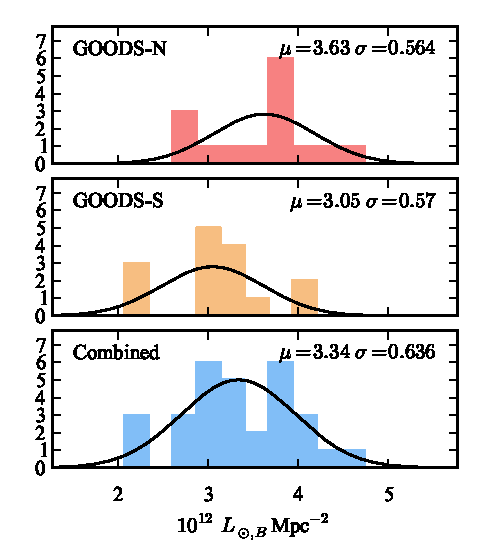
\includegraphics{figures/clrate/bkghist_all_V.eps}%
\includegraphics{figures/clrate/bkghist_all_S.eps}
\includegraphics{figures/clrate/bkghist_all_G.eps}%
\includegraphics{figures/clrate/bkghist_all_A.eps}
\caption[Distribution of luminosity density in GOODS
fields.]{Distribution of luminosity density in GOODS fields, with
galaxy selection and $K$-corrections applied for cluster V ($z=0.91$,
\emph{upper left}), cluster S ($z=1.07$, \emph{upper right}), cluster G 
($z=1.26$, \emph{lower left}), and cluster A ($z=1.45$, \emph{lower
right}). \label{fig:bkghist_all}}
\end{figure}

We select 30 non-connected circular regions (15 in each of GOODS North
and South) of radius $1'.4$, similar to the size of the cluster
fields.  ($1'.4$ corresponds to 0.654, 0.697, and 0.711 Mpc at
$z=0.9$, 1.2 and 1.5, respectively.)  The distribution of luminosity
densities in these 30 regions is shown for four example clusters in
Figure~\ref{fig:bkghist_all}. Because the same 30 regions are used for
each cluster, the resulting distributions are quite similar, though
not identical because of the different selections and $K$-corrections
used.  The average luminosity density of these fields is taken as the
``background'' luminosity for the cluster, and the standard deviation
(typically 15 -- 20 \% of the average) is taken as the error in this
background luminosity due to variations between fields.

We have implicitly assumed that the GOODS average accurately
represents the cosmic average. GOODS incorporates only two widely
separated fields. As a result, the average luminosity density may
differ from the cosmic average due to variations in large scale
structure. As a rough estimate of the cosmic variance, we compare the
two GOODS fields.  The average luminosity density of the GOODS-North
regions is consistently higher than that of the GOODS-South regions by
15 -- 20\% (Fig.~\ref{fig:bkghist_all}). This means that the ``standard deviation'' of these two
samples of large scale structure is $\sim$8\%. We checked this using
the cosmic variance calculator made available
by \citet{trenti08a}\footnote{\url{http://casa.colorado.edu/~trenti/CosmicVariance.html}}. The
expected cosmic variance in galaxy number counts in the redshift
window $0.7 < z < 1.7$ for one GOODS field is approximately $\sim$6\%,
in good agreement with our na\"ive estimate. Conservatively, we take
$8\%$ as the cosmic variance for one GOODS field. For
the \emph{average} of the North and South fields, this implies a
cosmic variance of $8\%/\sqrt{2} \sim 6\%$.

One might be additionally concerned that the ``background'' in the
cluster fields is biased higher than the cosmic average because
clusters form in regions of large-scale overdensities. However, each
cluster field is a ``pencil-beam'' galaxy survey, so the vast majority
of non-cluster galaxies will not be associated with the high-density
region in which each cluster formed.
